\chapter{Hoare-Style Verification}\label{ch:syntax}
While the methodology presented in the previous chapter
for verifying \gls{memuse} works well, it is not ideal.
The need to manually formulate regions
and the amount of work required for developing invariants
reduces potential scalability.

In order to deal with those downsides,
this \lcnamecref{ch:syntax} introduces the concept of \glspl[prereset]{fmuc}
generated by untrusted, informal tools.
\Glspl{fmuc} consist of two main components:
theorems on \gls{memuse} and \emph{proof ingredients}.%
\index{proof!ingredient}
The proof ingredients are assumptions on memory layout,
control flow information, and invariants
generated to reduce the amount of work required from end users.

Certificate generation is presented in \cref{se:fmuc_gen},
while the process of verification in \gls{isabelle} is documented in \cref{se:fmuc_ver}.
A full example of \gls{fmuc} usage can then be found in \cref{se:syntax_example}.
That example could theoretically overwrite
its own return address due to its pointer arguments, causing \gls{cfi} issues.
The associated \gls{fmuc} provides preconditions to prevent such cases
along with a formal proof of return address preservation under those conditions.
Following the example in \cref{se:xen} is an in-depth case study
on the Xen Project hypervisor \autocite{chisnall2008definitive}.
In total, \glspl{fmuc} were generated and proofs discharged in \gls{isabelle}
for 251 Xen functions.

\begin{comment}
  My primary contributions to the certificate generation and verification approach%
  \index{certificate}
  presented in this chapter include the Hoare rules developed
  for \gls{memuse} as well as the \gls{vcg} used to apply those rules
  to \gls{scf} in \gls{isabelle} (\cref{se:fmuc_ver}).
  I also greatly expanded the code for full translation of the \glspl{fmuc} into the \gls{isabelle}[/HOL] language and helped adapt the \gls{scf} into a form suitable for verification in \gls{isabelle} (\cref{isabelle_scf}).
  Additionally, I contributed to invariant generation (\cref{sse:inv_gen})
  and performed much of the verification work for our large case study,
  presented in \cref{se:xen}.
\end{comment}

\section{\Glsfmtshort{fmuc} Generation}\label{se:fmuc_gen}
\begin{figure*}
  \centering
  \begin{tikzpicture}[gnode/.style={draw, rounded corners, text centered}]
    \graph[grow right=2.88815cm]{
      Assembly[gnode] ->[dashed]
      "Control\\Flow\\Graph"[gnode,align=center] ->["\ref{sse:cfg_extract}"]
      "Syntactic\\Control\\Flow"[gnode,align=center] ->["\ref{sse:syntax_symb}"]
      "Memory\\Regions\\and\\\glsxtrshortpl{mrr}"[gnode,align=center]
      ->["\ref{sse:inv_gen}"]
      Invariants[gnode] ->[dashed] Certificate[gnode];
    };
  \end{tikzpicture}
  \caption{Overview of \glsfmtshort{fmuc} generation}\label{fig:overview}
\end{figure*}

\Glspl{fmuc} require the assembly code of a program as input.
That source assembly could be obtained from a binary using a disassembler, such as \texttt{objdump},
IDA \autocite{ida}, Ghidra's decompiler \autocite{ghidra}, or Capstone \autocite{capstone}.
If source code is available, it could be generated directly by a compiler instead.
Each function specified for verification receives \pgls{fmuc};
those that are not included in the verification effort,%
\index{verification!effort}
including system calls and functions from dynamic libraries,
can be treated as black boxes,
the usage of which is described in \cref{sse:fmuc_comp}.

The general procedure for generating \glspl{fmuc}, laid out in \cref{fig:overview},
can be broken up into three main parts.
The first part involves control flow extraction from the supplied assembly
using \pgls{cfg} analysis similar to angr's CFGFast%
\index{angr!CFGFast}
\autocite{shoshitaishvili2016state},
ultimately producing \pgls{scf} (the details of which are presented
in \cref{sse:cfg_extract}).
Afterwards, per-basic block symbolic execution
is utilized to generate the set of memory regions
read and written by the function in question.
This was detailed in \cref{ch:symbolic_execution}.
To eliminate duplicates and produce \glspl{mrr}
showing which regions overlap or are enclosed or separate,
the region sets are then fed to the \gls{smt} solver \gls{z3} \autocite{de2008z3}.
Symbolic execution is also used in the process of generating
the pre- and postconditions for each basic block,
elaborated on in \cref{sse:inv_gen}.

With the exception of \gls{mrr} generation,
none of the steps in this procedure are included in the \gls{tcb}.
The process of verifying the generated \gls{fmuc} (see \cref{se:fmuc_ver})
will fail if there are issues in control flow extraction,
\gls{scf} generation, informal symbolic execution, or invariant generation.
\Gls{mrr} generation is an exception
because the \glspl{mrr} are formulated as assumptions,
and thus inconsistent \glspl{mrr} will result in vacuous proofs.
This is why the methodology relies on \gls{z3} for \gls{mrr} generation;
using a known-reliable tool greatly reduces the possibility of issues.

\subsection{Control Flow Extraction}\label{sse:cfg_extract}
%As described in \cref{se:hoare},
%in
In order to apply \pgls{vcg} that utilizes Hoare rules to verify a Hoare triple,
there must be some syntactic structure to apply those rules to.
This chapter uses a syntactic representation of control flow called \gls{scf}
in part for that purpose.
\Gls{scf} expresses assembly programs as a combination of basic blocks,
branches, loops, and function calls.
The following grammar provides a description of \gls{scf}
produced by the extraction code.
Each basic block is represented by the polymorphic type~$\beta$,
while branching conditions are represented using the polymorphic type~$\Phi$.
\begin{bnf}
  \bnfprod*{scf}{
    \bnfpn{scf}\bnfsp\bnfts{;}\bnfsp\bnfpn{scf}
    \bnfor\bnfts{Block}\bnfsp\bnftd{$\beta$}
    \bnfor\bnfts{Skip}
    \bnfor\bnfts{Continue}
    \bnfor\bnfts{Break}\bnfsp\bnfpn{br}
  } \\
  \bnfmore{
    \bnfor\bnfts{If}\bnfsp\bnftd{$\Phi$}
      \bnfsp\bnfts{Then}\bnfsp\bnfpn{scf}
      \bnfsp\bnfts{Else}\bnfsp\bnfpn{scf}
      \bnfsp\bnfts{Fi}
    \bnfor\bnfts{Loop}\bnfsp\bnfpn{scf}\bnfsp\bnfts{Pool}\bnfsp\bnfpn{res}
  } \\
  \bnfprod{br}{
    \bnftd{ID}\bnfor\bnfes
  } \\
  \bnfprod{res}{
    \bnfts{Resume}\bnfsp\bnfts{\{(}\bnftd{ID}\bnfts{,}
      \bnfpn{scf}\bnfts{),}\bnfsk\bnfts{\}}
    \bnfor\bnfes
  }
\end{bnf}
Loops in this formulation have no exit condition;%
\index{loop}
instead, they rely on having one or more internal \texttt{Break} statements,%
\index{loop!break}
which may have an identifier to indicate how the loop was exited, for termination.
\texttt{Continue}s function the same as in C,%
\index{loop!continue}
causing loop execution to skip to the next iteration.
For loops that have multiple exit points,
\texttt{Resume} statements provide different code to execute
based on which exit was taken as indicated by the \texttt{Break} identifier.

Notably, the above data structure does not explicitly contain
control flow statements such as \lstinline|goto| or \lstinline|throw|/\lstinline|catch|.
Unconditional jumps like \lstinline|goto|s make code harder to reason about
in a structured way and can be modeled by the existing syntactic constructs,
while structured \gls{eh} as used in \gls{cpp} is generally provided
by external function calls.%
\index{exception handling!function}
%(\cref{se:structured_exceptions}).
\begin{example}[\Glsfmtshort{scf} extraction]
  \Cref{fig:ex_cf} provides an example of \gls{scf} extracted from \pgls{cfg}.
  The \gls{cfg} in \cref{fig:ex_cf_cfg} can be seen to have two branching conditions
  that do not involve loops, one from $\ABB~0$ with condition~$f_0$
  and one from $\ABB~7$ with condition~$f_7$.
  This leads to if statements with those conditions
  being added to the \gls{scf} in \cref{fig:ex_cf_scf} after their respective blocks.
  The one loop present has two exit points.
  If condition~$f_1$ is false after execution of $\ABB~1$,
  the loop will exit to $\ABB~4$, while $\ABB~2$ will exit to $\ABB~3$ if~$f_2$ is false.
  This leads to the $\ABreak$ statements present in the extracted \gls{scf}
  in their respective conditional statements
  annotated with the IDs for their associated exit blocks.
  Those two exit points also result in the generation of a $\AWhileResume$ clause
  indicating where those $\ABreak$s exit to.
  \begin{figure*}
    \hspace*\fill
    \subcaptionbox{Example \glsfmtshort{cfg}\label{fig:ex_cf_cfg}}{
      \begin{tikzpicture}[->, node distance=0.75cm]
        \node[draw=none] (0) {0};
        \node[draw=none] (1) [below=of 0] {1};
        \node[draw=none] (2) [below=of 1]{2};
        \node[draw=none] (3) [below=of 2]{3};
        \node[draw=none] (4) [left=of 3, xshift=0.5cm, yshift=0.5cm]{4};
        \node[draw=none] (5) [below=of 3]{5};
        \node[draw=none] (6) [below=of 5, xshift=0.5cm, yshift=0.5cm]{6};
        \node[draw=none] (7) [right=of 1]{7};
        \node[draw=none] (8) [right=of 3, xshift=0.5cm, yshift=0.5cm]{8};
        \node[draw=none] (9) [right=of 5]{9};

        \path (0) edge node[left]{$f_0$} (1);
        \draw[rounded corners=2mm] (0) -|
        node[above, xshift=0.4cm, yshift=-0.9cm]{$\neg f_0$} (7);
        \path (1) edge [bend left] node[right]{$f_1$} (2);
        \draw[rounded corners=2mm] (1) -| node[left, yshift=-1.3cm]{$\neg f_1$} (4);
        \path (2) edge [bend left] node[left, xshift=0.1cm]{$f_2$} (1);
        \path (2) edge node[right]{$\neg f_2$} (3);
        \path (3) edge node[right]{} (5);
        \draw[rounded corners=2mm] (4) |- (5);
        \path (5) edge node[right]{} (6);
        \draw[rounded corners=2mm] (7) -| node[right, yshift=-1.3cm]{$\neg f_7$} (8);
        \path (7) edge node[left, yshift=-1cm]{$f_7$} (9);
        \draw[rounded corners=2mm] (8) |- (9);
        \path (9) edge node[right]{} (6);
      \end{tikzpicture}
    }
    \hfill
    \subcaptionbox{Syntactic Control Flow\label{fig:ex_cf_scf}}{
      \(\begin{array}{l}
        \ABB~0\ASeq* \\
        \AIf~f_0~\AThen \\
        \ind{4ex}\AWhile \\
        \ind{8ex}\ABB~1\ASeq* \\
        \ind{8ex}\AIf~f_1~\AThen \\
        \ind{12ex}\ABB~2\ASeq* \\
        \ind{12ex}\AIf~f_2~\AThen~\AContinue~\AElse~\ABreak~2~\AFi \\
        \ind{8ex}\AElse \\
        \ind{12ex}\ABreak~1 \\
        \ind{8ex}\AFi \\
        \ind{4ex}\AOd~\AWhileResume~\{(2,\ABB~3),(1,\ABB~4)\}\ASeq* \\
        \ind{4ex}\ABB~5 \\
        \AElse \\
        \ind{4ex}\ABB~7\ASeq* \\
        \ind{4ex}\AIf~f_7~\AThen~\ASkip~\AElse~\ABB~8~\AFi\ASeq* \\
        \ind{4ex}\ABB~9 \\
        \AFi\ASeq* \\
        \ABB~6
      \end{array}\)
    }
    \hspace*\fill
    \caption{Example of control flow extraction}\label{fig:ex_cf}
  \end{figure*}
\end{example}

\subsubsection{Restrictions}
There two important restrictions on the current control flow extraction approach,
the more severe of which is the lack of support for indirect branching.
The \gls{cfg} analysis done by the current extraction algorithm
is not strong enough to handle indirect branching at the moment.
In some cases, the set of possible branches can be determined based on the
local function context, but the result of an indirect branch is often based off of input arguments, as well. Even if the result set
might be determinable with static analysis, it would have to be interprocedural,
and branch destinations based on external input cannot be determined.

Finally, as the if-then-else statement provides the sole form of
branching control flow, the algorithm is not optimal
due to the duplication of blocks to fit less structured control flow
into a more structured model. In the worst case,
it can result in \gls{scf} explosion, described below.

\subsubsection{\Glsfmtshort{scf} Explosion}\label{sse:scf_explode}
The algorithm is not optimal in terms of generated \gls{scf} size
as certain basic blocks may be duplicated.
There are two situations where basic block duplication occurs,
one less common than the other.
The less common situation is when loop having multiple entry points,
which can occur in situations that involve less-structured control flow,
such as a \gls{c} program that jumps into a loop using \texttt{goto}.
Such situations are relatively uncommon, even in optimized code.
If it does happen, the entire loop must be duplicated.
The more common situation, by contrast, involves complex conditional branching
that can occur even without loops.
\begin{example}[\Glsfmtshort{scf} explosion]
  \Cref{fig:ex_nonopt} shows a small example of branching control flow
  that results in $\ABB~3$ being duplicated.
  That block could itself be an even more complicated subgraph,
  possibly leading to exponential code duplication.
  \begin{figure*}
    \hspace*\fill
    \subcaptionbox{\Glsfmtshort{cfg}}{
      \begin{tikzpicture}[->, node distance=0.75cm]
        \node[draw=none] (0) {0};
        \node[draw=none] (1) [right=of 0] {1};
        \node[draw=none] (2) [right=of 1] {2};
        \node[draw=none] (3) [right=of 2] {3};
        \node[draw=none] (4) [right=of 3] {4};

        \path (0) edge node[below]{$f_0$} (1);
        \path (0) edge [bend left] node[above]{$\neg f_0$} (4);
        \path (1) edge node[above]{$f_1$} (2);
        \path (1) edge [bend right] node[below]{$\neg f_1$} (3);
        \path (2) edge node[above]{$f_2$} (3);
        \path (2) edge [bend right] node[below]{$\neg f_2$} (4);
        \path (3) edge (4);
      \end{tikzpicture}
    }
    \hfill
    \subcaptionbox{\Glsfmtshort{scf}}{
      \(\begin{array}{l}
        \ABB~0; \\
        \AIf~f_0~\AThen~\ABB~1; \\
        \ind{4ex}\AIf~f_1~\AThen~\ABB~2; \\
        \ind{8ex}\AIf~f_2~\AThen~\ABB~3 \\
        \ind{8ex}\AElse~\ASkip~\AFi \\
        \ind{4ex}\AElse~\ABB~3~\AFi \\
        \AElse~\ASkip~\AFi; \\
        \ABB~4
      \end{array}\)
    }
    \hspace*\fill
    \caption{Example of code duplication}\label{fig:ex_nonopt}
  \end{figure*}
\end{example}

\subsection{Symbolic Execution for Generation}\label{sse:syntax_symb}
In \cref{sse:cfg_extract}, the semantics of assembly were expressed%
\index{semantics!assembly}
in terms of control flow between basic blocks.
This section now covers the symbolic execution of those individual blocks.
The Haskell symbolic execution engine
takes as input a data structure of type $\scf(B,E_F)$,
which is formulated over basic blocks,
and produces $\scf(\powerset(\gls{assign}),\gls{esp})$,
which is formulated over sets of assignments.
It keeps track of all used memory regions,
both the actual regions used by instructions as well as merged regions,
in order to supply those regions as part of an \gls{fmuc}.

\subsubsection{Generating Memory Region Relations}
Because symbolic execution uses symbolic state,
the relations of enclosure, separation, and overlap,
defined in \cref{memory_aliasing}, must be determined for symbolic expressions.
Unfortunately, there is no single solution, no one decision procedure,
that can determine these properties for all symbolic expressions automatically.

As an example of the potential issues that can occur,
take the completely symbolic regions $r_0=\region{a_0}{s_0}$
and $r_1=\region{a_1}{s_1}$.
Without additional information, we cannot determine any relations for these regions.
If they are \emph{possibly} different then they must be treated as different regions,
while if they \emph{necessarily} overlap
then they must be treated as a single merged region.

To deal with such symbolic issues,
the three aforementioned relations of enclosure, separation, and overlap
are formulated as \gls{smt} problems.
The \gls{smt} formulations are negations
of the equations presented in \cref{def:sep,def:enc};
the result states the property holds if the resultant problem is \emph{unsatisfiable}.
These \gls{smt} problems can be solved by \gls{z3} \autocite{de2008z3}
for a wide range of expressions over bitvectors
using the \inlineisabelle{QF_UFBV} logic \autocite{smtlib:bitvector-logic,smtlib:bitvector-theory}.
\Gls{z3} is also used in this work for determining the sign of two values
in the region merge algorithm, originally presented in \cref{def:merge}.
Additionally, reads of overlapping regions may require merging
and separation analysis as described in \cref{memory_aliasing},
so they also rely on \gls{z3}.

The result of evaluating the above \gls{smt} problems
over all pairs of memory regions for a basic block, each region being given a unique ID,
is two sets with element type $\gls{nat}\times\gls{nat}$, $\var{enc}$ and $\var{ovl}$.
Every element $(i_0,i_1)$ in $\var{enc}$ indicates that the region with ID~$i_0$
is enclosed by the region with ID~$i_1$.
Every element $(i_0,i_1)$ in $\var{ovl}$ indicates that the two regions with those IDs
overlap.
Those two sets are the \glspl{mrr} for the block,
and using them as assumptions allows for efficient execution of the rewrite rules
in \cref{memory_rewrite}.

\subsection{Invariant Generation}\label{sse:inv_gen}
Invariants, formalized as sets of assignments of the aforementioned type~\gls{assign},
\index{invariant}
are generated by starting from a precondition for the entry point of the function
and \emph{propagating} it throughout.%
\index{invariant!propagation}

The initial precondition of the function as a whole is generated
by including initial symbolic values for all registers that are read
before they are written as well as all used memory regions
that are not enclosed in another.
The concrete initial value of the instruction pointer, \rip,
must also be included,
and the (symbolic) address to return to after function completion
must be indicated as stored on the stack.
In Haskell, the conditions in question are represented as sets of assignments.
\begin{example}[Initial invariant]
  To reuse \cref{ex:simple}, its initial precondition would be:
  \begin{equation}
    \phi=\{\mathrip\coloneqq\mathtt{a0},
    \mathrsp\coloneqq\rspo,
    \region{\mathrsp-8}{8}\coloneqq v_0,
    \region{\mathrsp}{8}\coloneqq\retaddr\}.
  \end{equation}%
  \nomenclature{$\phi$}{Denotes a generated invariant}
\end{example}
Propagation requires performing \emph{substitution},%
\index{invariant!substitution}
which is defined over assignments, state parts, and expressions,
all with respect to invariant~$\phi$.
\begin{subequations}
  \begin{align}
    \subst(\phi,\var{sp}\coloneqq v) &= \subst(\phi,\var{sp})\coloneqq\subst(\phi,v)\\
    \subst(\phi,\var{sp}) &= \text{if }\exists v\cdot(\var{sp},v)\in\phi
    \text{ then }v\text{ else }\var{sp} \\
    \subst(\phi,e_0\bop e_1) &= \text{if }\exists v\cdot(e_0\bop e_1,v)\in\phi
    \text{ then }v\text{ else }\subst(\phi,e_0)\bop\subst(\phi,e_1) \\
    \text{unary ops} &= \dotso \notag \\
    \text{ternary ops} &= \dotso \notag
  \end{align}
\end{subequations}%
\nomenclature[operator]{$\bop$}{Denotes an arbitrary binary operator}

\Cref{algo:prop} performs invariant propagation.
Each block is modified by applying all applicable substitutions
with respect to~$\phi$.
Invariant~$\phi$ is then modified based off of the semantics of the block.%
\index{semantics}
Treating~$\alpha$ as the set of assignments in the block,
$\phi$ is modified by taking the subset of substitutions
where the substitutees are overwritten by~$\alpha$
and combining them with the subset of substitutions
that were completely unmodified by any assignment in~$\alpha$:
\begin{equation}
  \post(\phi,\alpha)\footnote{%
    This is a different $\post$ from that used to identify \gls{cfg} block children.
  }\equiv\{(v,e)\mid(v\coloneqq e\in\alpha\land(v,\_)\in\phi)
  \lor((v,e)\in\phi\land(v,e)\text{ is unmodified by }\alpha)\}.
\end{equation}
\begin{example}[Invariant propagation]
  Once again consider \cref{ex:simple}.
  Propagation of the initial precondition through the single basic block
  produces the following postcondition:
  \begin{equation}
    \begin{split}
      \phi=\{\mathrip &\coloneqq\retaddr, \\
      \mathrsp &\coloneqq\rspo+8, \\
      \region{\rspo-8}8 &\coloneqq\mathtt{0xAABBCCDD}\concat
      \takebits{31,16}v_0\concat\mathtt{0xEEFF}, \\
      \region{\rspo}8 &\coloneqq\retaddr\}.
    \end{split}
  \end{equation}
\end{example}
\begin{algorithm}
  \caption{Invariant propagation}\label{algo:prop}
  \begin{algorithmic}
    \Require{Input is of type $\scf(\powerset(\gls{assign}),\gls{esp})$}
    % only \glsentryshort works for some reason
    \Ensure{Output is a tuple of possibly-updated~$\phi$
      and \glsentryshort{scf} updated with current~$\phi$:
      $\gls{assign}\times\scf(\powerset(\gls{assign}),\gls{esp})$}
    \Function{prop}{$\phi,\ABB~\alpha$}
      \State $\phi'\gets\post(\phi,\subst(\phi,\alpha))$
      \State\Return $(\phi',\ABB~(\alpha\text{ annotated with }\phi))$
    \EndFunction
    \Function{prop}{$\phi,\alpha_0\ASeq \alpha_1$}
      \State $(\phi',\alpha_0')\gets\Call{prop}{\phi,\alpha_0}$
      \State $(\phi'',\alpha_1')\gets\Call{prop}{\phi',\alpha_1}$
      \State\Return $(\phi'',\alpha_0'\ASeq \alpha_1')$
    \EndFunction
    \Function{prop}{$\phi,\AIf~f~\AThen~\alpha_0~\AElse~\alpha_1~\AFi$}
      \State $(\phi_0,\alpha'_0)\gets\Call{prop}{\phi,\alpha_0}$
      \State $(\phi_1,\alpha'_1)\gets\Call{prop}{\phi,\alpha_1}$
      \State $\phi'\gets\phi_0\cap\phi_1$
      \State\Return $(\phi',\AIf~\subst(\phi,f)~\AThen~
        \alpha'_0~\AElse~\alpha'_1~\AFi)$
    \EndFunction
    \Function{prop}{$\phi,\AWhile~\alpha~\AOd$}
      \State $(\phi',\alpha')\gets\Call{prop}{\phi,\alpha}$
      \If{$\phi\subseteq\phi'$}%
        \nomenclature[operator]{$\subseteq$}{Indicates subset relation}
        \State\Return $(\phi,\AWhile~\alpha'~\AOd)$
      \Else
        \State\Return $\Call{prop}{\phi\cap\phi',\AWhile~\alpha~\AOd}$
      \EndIf
    \EndFunction
    \Function{prop}{$\phi,\AWhileResume~\var{resumes}$}
      \ForAll{$\alpha_i\in\var{resumes}$}
        \State $(\phi'_i,\alpha'_i)\gets\Call{prop}{\phi,\alpha_i}$
      \EndFor
      \State $\phi''\gets\bigcap\phi'$
      \State\Return $(\phi'',\AWhileResume~\Call{zip}{i,\alpha'})$
    \EndFunction
    \Function{prop}{$\phi,\alpha$}\Comment{Default case}
      \State\Return $(\phi,\alpha)$
    \EndFunction
  \end{algorithmic}
\end{algorithm}
Invariant propagation is straightforward for sequencing and if statements,
with sequencing simply chaining invariant propagation
and if statements producing an invariant that is the common result
of propagating the initial invariant down both branches.

In contrast, a loop with body~$\alpha$ requires continual propagation
until the invariant~$\phi$ stabilizes, possibly by becoming~$\varnothing$.%
\nomenclature{$\varnothing$}{The empty set}
This stabilization is identified
by checking if~$\phi$ is a subset of its propagated self.
If it is, then \gls{prop} returns the propagated~$\phi$
and a new loop with the propagated body.
Otherwise,
the original loop is propagated again with the intersection of~$\phi$
and its propagated self.
This process effectively computes the loop invariant
as the greatest subset of the initial invariant
that is preserved by execution of the loop body.
For loops that have multiple exits,
each exit's resume is propagated with the invariant at the point of exit evaluation.
In a similar fashion to the process for if statements,
the invariants that result from individual resume propagation
are intersected to produce a singular invariant for all resumes,
which is then returned along with all of the propagated resumes.

\section{\Glsfmtshort{fmuc} Verification}\label{se:fmuc_ver}
This section presents verification of \pgls{fmuc} as shown in \cref{fig:verify},
one of the primary contributions for this chapter as mentioned in its preamble.
Both the \gls{fmuc} and the original assembly are loaded into \gls{isabelle}[/HOL],
where the \gls{memuse} theorem is then proven using the proof ingredients
provided by the \gls{fmuc}.
By this method, which requires a step function
that models the semantics of the assembly instructions
and a process to apply it repeatedly,
the \gls{fmuc}['s] \gls{memuse} Hoare triple can be verified.

\begin{figure*}
  \centering
  \begin{tikzpicture}[->, every node/.style={
    draw,
    rounded corners,
    text width=3cm,
    text centered,
    minimum height=1.5cm
  }]
    \node (a) {\gls{isabelle}[/HOL]};
    \node[above left=of a] (b) {Assembly};
    \node[below left=of a] (c) {Certificate};
    \node[right=1.5cm of a] (d) {OK/unproven};

    \draw (b) -- (a.north west);
    \draw (c) -- (a.south west);
    \draw (a) -- (d);
  \end{tikzpicture}
  \caption{Overview of \glsfmtshort{fmuc} verification}\label{fig:verify}
\end{figure*}

% \glsentryname doesn't handle post-insertion so no point in using it here
\subsection{Syntactic Control Flow in \texorpdfstring{\gls{isabelle}[/HOL]}{Isabelle/HOL}}\label{isabelle_scf}
As described previously, \gls{scf} is a representation of the control flow of a function
in terms of syntactic structures such as basic blocks,
loops, and if-then-else statements.
While very similar to the \gls{scf} used when generating \glspl{fmuc},
there are some modifications that must be made when the generated \glspl{scf}
are to be loaded into \gls{isabelle}[/HOL].
These modifications are required due to subtle differences in the semantics
of the generating tool versus the verifying tool,
and are required to properly support the Hoare rules
described in \cref{scf_hoare} below.

In the \gls{isabelle}[/HOL] representation,
there are no \texttt{Break}s or \texttt{Continue}s;
any occurrences of such statements are translated to \texttt{Skip}.
This does mean that programs that cannot be easily transformed
such that that translation does not modify the overall semantics
are not easily handled in this framework.
However, none of functions encountered in the case study presented in \cref{se:xen}
had that issue, so it does not appear to be a significant drawback.

Additionally, loops in the \gls{isabelle}[/HOL] \gls{scf} syntax do rely on a explicit exit condition.
This condition is simply the precondition of the entry block of the loop
as generated using the methodology in \cref{sse:inv_gen}.

Another important difference is that basic blocks in \gls{isabelle} take the form $\ABB~\Block*{n}{a}{i}$,
where~$n$ indicates the number of instructions in the block,~$a$ is the address
of the last instruction in the block, and~$i$ is an ID
that uniquely identifies the block in the current \gls{scf}.
This style is used to assist with the symbolic execution methodology described in
\cref{sse:syntax_ver_symb}.

Finally, to properly handle function calls in the \gls{isabelle}[/HOL] syntax,
the analyzed \glspl{cfg} are preprocessed prior to performing extraction
in order to isolate \inlineasm{call} instructions into their own basic blocks.
% Freek did the preprocessing but I did all the rest.
These single-instruction blocks are then translated into \texttt{Call}~$f$ entries
in the \gls{isabelle}[/HOL] \gls{scf}, where~$f$ is the textual label of the function called.
This allows for proper matching with the Hoare rules presented below.

\subsection{Symbolic Execution for Verification}\label{sse:syntax_ver_symb}
\Cref{cfg_symb_exec} previously presented a formal symbolic execution engine
based on the machine model described in \cref{se:machine_model}.
It provides a function \gls{run} that describes the symbolic execution of
blocks in a control flow graph.

The formal function for block-level symbolic execution presented in this chapter,%
\index{symbolic!execution}
by contrast, is a \emph{transition relation}%
\index{transition relation} formulated as
\begin{equation*}
  \execblock:\gls{nat}\times W\times\gls{nat}\times S\times S\rightarrow\gls{bool}.
\end{equation*}
Its inputs are the number of instructions left to execute in the block,
the address of the last instruction in the block, the block's ID,
the current state~$\sigma$, and an ending state~$\sigma'$.
Its result is true if and only if execution
starting from the current instruction in state~$\sigma$
and running to the ending address can produce state~$\sigma'$.
The other arguments are used to ensure termination and block matching.
Undefined behavior, such as null-pointer dereferencing,
is modeled by relating the state in which it occurs to any successor state
supplied with it.

The internal step function has type $\gls{step}:A\times\gls{nat}\times S\rightarrow S$,
with its first argument being an instruction, its second being the size of the instruction,
and its third being the current state.
The function returns the state after instruction execution,
incrementing \rip\ by the supplied size
if it was not changed by a control flow instruction instead.

% TODO: provide the detail of the $\exec$ function if time permits
The $\execblock$ function is used internally by another transition relation,
this one for the symbolic execution of entire \glspl{scf}:
$\exec:\var{SCF}\times S\times S\rightarrow\mathbb{B}$.
That function recurses through \pgls{scf}
and checks $\execblock$ on every block it finds,
performing the necessary state transformations to deal with the semantics of
the individual \gls{scf} components encountered.
Any loops encountered are dealt with using \pgls{lfp} construction.
This means that, if there are any infinite loops present,
the function will have no related successor states.
The only matching state would be $\infloop$.
Strictly speaking, $\exec$ is not actually executed when used in \gls{fmuc} proofs;
it exists to allow proving the correctness
of the Hoare rules shown below in \cref{scf_hoare}.

Unlike the symbolic execution for generation,
this symbolic execution methodology is implemented fully in \gls{isabelle}[/HOL],
meaning that every rewrite rule has been formally proven correct.

\subsection{Per-Block Verification}\label{sse:per-block}
The verification methodology presented here occurs
by first verifying the functionality of each basic block in the corresponding function.
This is done for each block by proving the lemma shown below,
using the $\exec$ function from the previous section.
To do this, however, a formal notion of \emph{\gls{memuse}}
with respect to state changes is required.
\begin{definition}[Memory usage with respect to state changes]\label{def:mem_preserve}
  The set of memory regions~$M'$ characterizes \gls{memuse} with respect to
  the change from some state~$\sigma$ to some other state~$\sigma'$
  if and only if every byte outside of the regions in~$M'$ is the same in both states.
  The addresses of those bytes are represented by the variable~$a$.

  This is formally expressed as:
  \begin{equation}
    \usage(M',\sigma,\sigma')\equiv\forall a\cdot(\forall r\in M'\cdot\region{a}1\gls{separate}r)
    \longrightarrow\readmemS{\sigma}a{1}=\readmemS{\sigma'}a{1}.
  \end{equation}
\end{definition}

Using \cref{def:mem_preserve}, each block gets a lemma of the form
\begin{equation}
  P(\sigma)\longrightarrow\execblock(n,a,i,\sigma,\sigma')\land
  Q(\sigma')\land\usage(M(\sigma),\sigma,\sigma').\label{eq:block_lemma}
\end{equation}
Note that~$M$ is a state-dependent function.
Every generated version of \cref{eq:block_lemma} is discharged
with an \gls{isabelle}[/HOL] proof method written in Eisbach \autocite{matichuk2016eisbach},
\gls{isabelle}'s proof automation language.
For each block, the method takes the block-related proof ingredients
from the \gls{fmuc} and runs symbolic execution
to prove the postcondition and thus establish \gls{memuse} for the block.
The open variables $P$, $Q$, $n$, $a$, $i$, and $M$ are all provided by the \gls{fmuc}.
No user interaction is required outside of cases where semantics
for specific instructions are unavailable or the \gls{isabelle} libraries in use
do not have the right simplification lemmas for automatic reasoning.
Those cases are rare and become rarer as more relevant lemmas are developed,
so for basic blocks, the proof is essentially automated.

\subsection{Function Body Verification}
While symbolic execution works well to establish \gls{memuse} on the level of basic blocks,
the goal of this verification effort is to formally establish \gls{memuse}
on the function level. This section describes that process,
which occurs after the individual blocks have had their semantics and \gls{memuse} derived
and relies on \gls{hoare-logic}. % (described in \cref{se:hoare}).

\subsubsection{Hoare Rules}\label{scf_hoare}
The Hoare triple formulation used for this work, $\htriple*{P}f{Q}M$,
resembles traditional Hoare triples a bit more than the version from \cref{ch:cfg},%
\index{Hoare!triple}
as rather than a halting condition
it takes a syntactic representation of the program, an \gls{scf}.
Unlike traditional Hoare triples, however,
it also explicitly contains the set of memory regions,~$M$,
that contain the areas of memory read and written by the program the \gls{scf} encodes.
Syntactic structure is required because \gls{hoare-logic} is a Hoare-style approach.
\begin{definition}[Hoare triple for \glsfmtshort{scf}]\label{def:preserve}
  \begin{equation}
    \htriple*{P}f{Q}{M}\equiv
    \forall\sigma~\sigma'\cdot P(\sigma)\land\exec(f,\sigma,\sigma')\longrightarrow
    Q(\sigma')\land\usage(M,\sigma,\sigma')
  \end{equation}
\end{definition}
The above definition states the following:
if precondition~$P$ holds on the initial state~$\sigma$
and~$\sigma'$ would be the result of symbolically executing the \gls{scf}~$f$,
postcondition~$Q$ will hold on the produced state
and any values stored in the regions of memory outside set~$M$ remain unchanged.

While \cref{def:preserve} focuses on the regions written to,
the regions read must also be included as symbolic execution
relies on those regions being included.
Without them, proofs that require symbolically executing
the related instructions will not complete.

\begin{figure*}
  \centering
  \subcaptionbox{Introduction rule\label{fig:intro-rule}}{
    \AxiomC{$\begin{multlined}
      \forall\sigma~\sigma'\cdot P(\sigma)\longrightarrow \\
      \execblock(n,a,i,\sigma,\sigma')\land{} \\
      Q(\sigma')\land\usage(M(\sigma),\sigma,\sigma')
    \end{multlined}$}
    \AxiomC{$M'=\{r\mid\exists\sigma\cdot P(\sigma)\land r\in M(\sigma)\}$}
    \BinaryInfC{$\htriple*{P}{\ABB~\Block*{n}{a}{i}}{Q}{M'}$}
    \DisplayProof
  }

  \subcaptionbox{Sequence rule}{
    \AxiomC{$\htriple*{P}f{Q}{M_1}$}
    \AxiomC{$\htriple*{Q}g{R}{M_2}$}
    \AxiomC{$M=M_1\cup M_2$}
    \TrinaryInfC{$\htriple*{P}{f\ASeq g}{R}{M}$}
    \DisplayProof
  }

  \subcaptionbox{Conditional rule}{
    \AxiomC{$\htriple*{P\land B}f{Q_1}{M_1}$}
    \AxiomC{$\htriple*{P\land\neg B}g{Q_2}{M_2}$}
    \AxiomC{$Q_1\lor Q_2\longrightarrow Q$}
    \AxiomC{$M=M_1\cup M_2$}
    \QuaternaryInfC{$\htriple*{P}{\AIf~B~\AThen~f~\AElse~g~\AFi}{Q}{M}$}
    \DisplayProof
  }

  \subcaptionbox{While rule\label{fig:hoare-loop}}{
    \AxiomC{$\htriple*{I\land B}f{I'}{M}$}
    \AxiomC{$I'\longrightarrow I$}
    \AxiomC{$I\land\neg b\longrightarrow Q$}
    \TrinaryInfC{$\htriple*{I}{\texttt{While}~B\texttt{ DO }f\texttt{ OD}}{Q}{M}$}
    \DisplayProof
  }
  \hfill
  \subcaptionbox{Skip rule}{
    \AxiomC{$M=\varnothing$}
    \AxiomC{$P\longrightarrow Q$}
    \BinaryInfC{$\htriple*{P}\ASkip{Q}{M}$}
    \DisplayProof
  }\hspace*\fill

  \subcaptionbox{Resume rule}{
    \AxiomC{$\forall {0\leq j\leq n}\cdot\htriple*{P}{a_j}{Q_j}{M_j}$}
    \AxiomC{$(\bigvee_{0\leq j\leq n} Q_j)\longrightarrow Q$}
    \AxiomC{$M = \bigcup_{0\leq j\leq n}M_j$}%
    \nomenclature[operator]{$\bigcup$}{Repeated union over a sequence or set of sets, akin to sum/product notation}
    \TrinaryInfC{$\htriple*{P}{\AWhileResume\{(i_0,a_0),\dotsc,(i_n, a_n)\}}{Q}{M}$}
    \DisplayProof
  }

  \hspace*\fill
  \subcaptionbox{Precondition weakening\label{fig:hoare-weaken}}{
    \AxiomC{$P\longrightarrow P'$}
    \AxiomC{$\htriple{P'}b{Q}{M}$}
    \BinaryInfC{$\htriple{P}b{Q}{M}$}
    \DisplayProof
  }
  \hfill
  \subcaptionbox{Postcondition strengthening}{
    \AxiomC{$Q'\longrightarrow Q$}
    \AxiomC{$\htriple*{P}b{Q'}{M}$}
    \BinaryInfC{$\htriple*{P}b{Q}{M}$}
    \DisplayProof
  }\hspace*\fill
  \caption{Hoare rules for \gls{memuse}}\label{fig:rules}
\end{figure*}

\subsubsection{The Introduction Rule}
This rule, depicted in \cref{fig:intro-rule},
is the rule that ties the per-block verification to the function-body verification.
The first assumption requires the symbolic execution method be run
from a universally quantified initial symbolic state~$\sigma$ that satisfies the precondition.
As long as any resulting state~$\sigma'$ satisfies the postcondition~$Q$,
the set of memory regions~$M$ generated for the block should be correct.

The second assumption is required because of an important subtlety:
the regions generated in the~\gls{fmuc} are state dependent.
As previously stated,
the~$M$ for a block is actually a function based on the block's initial state:
its regions depend on the values stored in memory.
However, it makes no sense to express the regions used by individual blocks
within a larger function in terms of their own individual initial state alone.
It would be unsound for regions that depend on values calculated
in the middle of the function to be expressed solely in terms of the initial state.
As such,
the Hoare triples are defined over a state-independent set of memory regions,~$M'$.
That set is obtained for each block
by taking the generated state-dependent set of memory regions
and applying that set to any state that satisfies the current invariant.

\subsubsection{The Other Rules}
While the introduction rule for basic blocks
is the ultimate target of our Hoare rule application process,
the rest of the rules are required to decompose the syntax above the level of blocks.
The remainder of \cref{fig:rules} describes those additional rules.
The Sequence, Conditional, and Resume rules are straightforward:
their ultimate memory region sets are the unions of the region sets of their constituents.
Note that the sequence rule is sound only because the memory predicates
are independent of state as discussed in \cref{sse:per-block}.

The while rule is based on a loop invariant,~$I$.
If the \gls{memuse} of one iteration of loop body~$f$
is constrained to set of memory regions~$M$,
then so is the \gls{memuse} of every other iteration.
This may sound counterintuitive,
so consider a simple C-like loop that starts from $i=0$ and iterates while $i<10$.
The body of this example loop contains single-byte array assignment operations
along the lines of $a[i]=v$.
Verification of the loop requires the loop invariant $I(\sigma)=i(\sigma)<10$.
The \gls{fmuc} of the loop body will have, as a state-dependent set of memory regions, $M(\sigma)=\{\region{a+i(\sigma)}1\}$, which is a single region of one byte.
If the \gls{hoare-logic} introduction rule were to be applied to the block
that is the body of the loop, the result would be as follows:
\begin{subequations}
  \begin{align}
    M' &= \{r\mid\exists\sigma\cdot I(\sigma)\land r\in M(\sigma)\} \\
    &= \{r\mid\exists\sigma\cdot i(\sigma)<10\land r=\region{a+i(\sigma)}1\} \\
    &= \{\region{a'}1\mid a\leq a'\le a+10\}
  \end{align}
\end{subequations}
The set~$M'$ contains the regions of memory used by the entire loop,
not just one iteration.
This is because the introduction rule applies the state-dependent set of memory regions
to any state that satisfies the invariant.
Thus, the strength of the generated invariants directly influences
the tightness of the overapproximation of \gls{memuse}
and of \gls{memuse} as a whole.
A weaker invariant, such as $i<20$, would result in a larger set of memory regions
by relaxing the constraints on symbolic addresses and,
for other situations, symbolic region sizes.

\begin{lstlisting}[
  gobble=2,
  float=*,
  language=Isabelle,
  caption=VCG step method,
  label=lst:vcg_step
]
  method vcg_step =
    ((rule htriples)+, rule blocks)+,
    (simp add: pred_logic Ps Qs)?, |\label{step_simp}|
    (((auto simp: eq_def)[])+)? |\label{step_auto}|
\end{lstlisting}
\begin{lstlisting}[
  gobble=2,
  float=*,
  language=Isabelle,
  caption=Main VCG method,
  label=lst:vcg
]
  method vcg uses scf =
    subst scf,
    vcg_step+
\end{lstlisting}
\subsubsection{Verification Condition Generation}\label{sse:vcg}
The \gls{vcg} presented here is a set of Eisbach proof methods,
the entry point of which is shown in \cref{lst:vcg}.
It is designed to automatically apply the proper \gls{hoare-logic} rules
as much as possible via the \inlineisabelle{vcg_step} method in \cref{lst:vcg_step},
driven by the formal \gls{scf} provided by the \gls{fmuc}.

Internally, \inlineisabelle{vcg_step} repeatedly applies one of the Hoare rules
from \cref{fig:rules} (excluding the While, strengthening, and weakening rules)
to the current state of the \gls{scf} until no more rules can be applied.
At that point, it assumes that the introduction rule has been applied,
resulting in a block goal being generated, and attempts to discharge that goal
using one of the lemmas generated for \cref{sse:per-block}.
This process is repeated until no more of the restricted set of rules can be applied
or the last rule application resulted in a non-block goal.
At that point, \cref{step_simp} cleans up any preconditions and postconditions
in the current goal.
The last step, \cref{step_auto}, then tries to eliminate as many goals as it can,
one at a time, with \gls{isabelle}'s basic \inlineisabelle{auto} method.
If there are no loops present in the \gls{scf} under consideration,
this method will complete the proof without any need for user interaction.

\begin{lstlisting}[
  gobble=2,
  float=*,
  language=Isabelle,
  caption=Alternate step method for $\AWhileResume$ clauses,
  label=lst:vcg_cases
]
  method vcg_step' =
    (rule htriples)+,
    simp,
    ((rule htriples)+, rule blocks)+,
    (simp add: pred_logic Ps Qs)?,
    (((auto simp: eq_def)[])+)?
\end{lstlisting}
\begin{lstlisting}[
  gobble=2,
  float=*,
  language=Isabelle,
  caption=VCG method for loops,
  label=lst:vcg_while,
  escapechar=*
]
  method vcg_while for P :: state_pred =
    ((rule htriples)+)?,
    rule HTriple_weaken[where P=P], *\label{step_weaken}*
    simp add: pred_logic Ps Qs,
    rule HTriple_while,
    vcg_step+,
    (simp add: pred_logic Ps Qs)+,
    (
      (vcg_step' | vcg_step)+,
      (simp+)?
    )?
\end{lstlisting}
In the case where loops are present,
the \gls{vcg} provides an alternate \inlineisabelle{vcg_while} method,
shown in \cref{lst:vcg_while}
that relies on the loop rule presented in \cref{fig:hoare-loop}.
That loop rule is structured such that
the majority of work required to support the loops
is identifying the preconditions of their exit blocks
and then supplying their disjunction to \inlineisabelle{vcg_while}.
This method relies on application of the weakening rule
presented in \cref{fig:hoare-weaken} on \cref{step_weaken}
to show that the postcondition of the block before entry implies the loop invariant.

The method \inlineisabelle{vcg_step'}, used within \inlineisabelle{vcg_while},
is provided for those cases where a loop has multiple exit points.
A $\AWhileResume$ statement will be present in such cases,
and the process of rule application and simplification must occur
in a slightly different order. On occasion, there will also be a loop that has a single
exit point but gets a $\AWhileResume$ statement anyway
due to how the control flow extraction algorithm is set up.
The process of dealing with such statements is roughly the same, however.

After application of \inlineisabelle{vcg_while},
nested loops and those with multiple exit points may require
additional applications of condition simplifying or plain \inlineisabelle{simp} usage
around further applications of \inlineisabelle{vcg_step}.
Nothing beyond that should be necessary.

Without exception, each of the proofs we produced
could be finished using standard, off-the-shelf \gls{isabelle}[/HOL] methods,
though finishing them was not always an automatic process.
The part that is usually the most involved,
defining the invariants (as seen in the previous chapter)
is taken care of by the \gls{fmuc} generation.
This leaves dealing with loops, particularly ones with multiple exit points,
as the biggest challenge for most situations.

\subsection{Composition}\label{sse:fmuc_comp}
In order to achieve a scalable verification methodology,
it must support some form of compositionality.

Consider the body of an already-verified function~$f$
with the following Hoare triple:
\begin{equation*}
  \htriple*{P_f}f{Q_f}{M_f}.
\end{equation*}
In order to reuse that function's proof in a compositional fashion,%
\index{function!composition}
it is treated as a black box.%
\index{function!black box}
Now consider the assembly of a function~$g$ that calls~$f$:
\begin{lstlisting}[style=x64, gobble=2, numbers=none]
  a0: push rbp
  a1: call f
  a2: pop  rbp
  a3: ret
\end{lstlisting}
$P$ and~$Q$ are the pre- and postconditions just before executing \inlineasm{call}
and just after it returns.
$P$ contains the equality $\readmem{\rspo^g-8}{8}=\rbpo^g$,
expressing that~$g$ has pushed the frame pointer \rbp%
\index{frame!pointer}
into its own local stack frame.%
\index{stack!frame}
The ultimate postcondition of~$g$
expresses that the callee-saved register \rbp\ is properly restored:%
\index{register!callee-saved}
$\mathrbp=\rbpo^g$.
That operation is indeed performed by \inlineasm{pop rbp}.
In order to prove proper restoration of \rbp,
a proof that function~$f$ did not overwrite any byte in the region%
\index{memory!region}
$\region{\rspo^g-8}{8}$ is required.
The proof must also show that~$f$ does not overwrite region $\region{\rspo^g}{8}$,
which stores the address~$g$ returns to.
That proof would be specific to this particular instance of calling~$f$.

Of course,~$g$ may not be the only function that calls~$f$.
It may even be called multiple times by the same function.
Every call has specific requirements on which memory regions must be preserved,
based on the calling context.
Thus, to be able to verify function~$f$ once
but reuse its proof for each call,
the proof must at least contain an overapproximation
of the memory written to by function~$f$.
This is exactly what \emph{separation
logic} \autocite{o2001local,reynolds2002separation,krebbers2017essence}%
\index{separation logic}
requires.
As described in \cref{sse:composition},
separation logic provides a \emph{frame rule} for compositional reasoning.%
\index{separation logic!frame rule}
Informally, this rule states that, if a program can be confined
to a certain part of state, properties of that program will carry over
when the program is used as part of a bigger system.

In order to achieve that same behavior specifically for \gls{memuse} verification,%
\index{memory!usage}
we developed the frame rule presented in \cref{fig:composition}.
This rule is used to prove that the \gls{memuse} of a caller function~$g$
is equal to the memory it itself uses, \emph{plus} the memory used by function~$f$.
It must have the following four assumptions.
First, that~$f$ has been verified for \gls{memuse},
with~$M_f$ denoting the memory regions~$f$ uses.%
\index{memory!region}
Second, that precondition~$P$ can be split up into two parts:
precondition~$P_f$, required to verify~$f$, and a separate part~$\psep$.
The separate part is specific to the specific call of the function
where the frame rule is applied.%
\index{separation logic!frame rule}
In the example above,~$P_\mathrm{sep}$ must contain the equality
$\region{\rspo^g-8}{8}=\rbpo^g$.
Third, the correctness of~$M_f$, the set of memory regions,
should suffice to prove that~$\psep$ is preserved.
This effectively means that, for the above example,~$M_f$
should not overlap with the two regions of~$g$.
Fourth and finally,~$\psep$ and~$Q_f$ should imply postcondition$~Q$.
\begin{figure*}
  \begin{prooftree}
    \def\defaultHypSeparation{\hskip.18in}
    \AxiomC{$\htriple*{P_f}{f}{Q_f}{M_f}$}
    \AxiomC{$P\longrightarrow P_f\land\psep$}
    \AxiomC{$\forall s~s'\cdot\begin{array}{l}
      (\usage(M_f,s,s')\land{} \\
      \psep(s))\longrightarrow\psep(s')
    \end{array}$}
    \AxiomC{$Q_f\land\psep\longrightarrow Q$}
    \QuaternaryInfC{$\htriple*{P}{\ACall f}{Q}{M_f}$}
  \end{prooftree}
  \caption{Frame rule for composition of \gls{memuse}}\label{fig:composition}
\end{figure*}

In practice, many functions will not be part of the assembly code under verification, such as dynamic library or system calls.
Those cases necessitate generating the assumptions required
to proceed with verification.
The following box notation supports those cases:
\begin{equation}
  \htriple*P{\fbox f}Q{M_f}\equiv
  \exists P_f~Q_f~\psep\cdot
  \text{all four assumptions of the frame rule are satisfied}.
\end{equation}
This assumption informally expresses that function~$f$ has been verified.
Its \gls{memuse}~$M_f$ is assumed to suffice to prove that
the states that satisfy precondition~$P$ lead to the states that satisfy
postcondition~$Q$.

\section{Full Example}\label{se:syntax_example}
This section presents an execution of the entire toolchain
on the example given in \cref{fig:example2-c}
as a summary of \cref{se:fmuc_gen,se:fmuc_ver}.
The~C code is provided solely for presentation,
as the only inputs to the \gls{fmuc} generation
are the assembly created by disassembling the corresponding binary%
\index{assembly}%
\index{assembly!dis-}%
\index{binary}
and a basic configuration file indicating which functions to analyze.
\Cref{fig:example2-scf} presents the generated \gls{scf}.
The example has one loop, which starts at instruction address \texttt{0x120}.%
\index{loop}
\begin{figure}
  \begin{subfigure}[b]{.53\linewidth}
    \begin{lstlisting}[language=C, gobble=6]
      int main(int argc, char** argv) {
        int* a = (int*)argv;
        int* b = (int*)(argv + 4);
        *(int*)(argv + 2) = *a + *b;
        *(char*)argv = 'a';

        int array[argc];
        for (int i = 0; i < argc; i++)
          array[i] = argv[i][0] * 2;

        if (is_even(argc))
          return array[argc];
        return array[0];
      }
    \end{lstlisting}
    \caption{C code}\label{fig:example2-c}
  \end{subfigure}%
  \hfill
  \begin{subfigure}[b]{.46\linewidth}
    \begin{equation*}
      \begin{array}{l}
        \ABB~\Block{1149}{120b}\ASeq* \\
        \AWhile \\
        \ind{2ex}\ABB~\Block{123e}{1244}\ASeq* \\
        \ind{2ex}\AIf~\var{SF}\neq\var{OF}~\AThen~\ABB~\Block{120d}{123a} \\
        \ind{4ex}\AElse~\ABreak~\AFi \\
        \AOd\ASeq* \\
        \ABB~\Block{1246}{1249}\ASeq* \\
        \ABB~\Block{124b}{124b}\ASeq* \\
        \ABB~\Block{1250}{1252}\ASeq* \\
        \AIf~\var{ZF}~\AThen~\ABB~\Block{1263}{1267} \\
        \ind{2ex}\AElse~\ABB~\Block{1254}{1261}~\AFi\ASeq* \\
        \ABB~\Block{1269}{1279}\ASeq* \\
        \AIf~\var{ZF}~\AThen~\ABB~\Block{1280}{1285} \\
        \ind{2ex}\AElse~\ABB~\Block{127b}{127b}~\AFi
      \end{array}
    \end{equation*}
    \caption{Syntactic control flow for the assembly}\label{fig:example2-scf}
  \end{subfigure}
  \begin{subfigure}{\linewidth}
    \begin{align*}
      M &=\{r_0=\region{\rspo}8, r_1=\region{\fso+40}8, r_2=\region{\rsio+36}4,
            r_3=\region{\rspo-8}8,\dotsc\} \\
      \var{MRR} &= \{r_0,r_1,r_2,r_3,\dotsc,r_{12}\}\text{ are separate}
    \end{align*}
    \caption{Some memory regions and their relations for block $\Block{123e}{1244}$}
  \end{subfigure}
  \begin{subfigure}{\linewidth}
    \begin{equation*}
      P_\mathtt{123e}(\sigma)=\begin{aligned}
        \mathrip            &= \mathtt{0x123e} \\
        \mathrbp            &= \rspo-8 \\
        \mathrdi            &= \rdio \\
        \mathrsp            &= \rspo-(88+16*((15+4*
          \gls{sextend}(\takebits{31,0}\rdio)/16)) \\
        \readmem{\rspo-40}8 &= \rspo-(85+16*((15+4*
          \gls{sextend}(\takebits{31,0}\rdio))/16))\gg 2\ll 2 \\
        \readmem{\rspo-48}8 &= \gls{sextend}(\takebits{31,0}\rdio)-1 \\
        \readmem{\rspo-56}8 &= \rsio+32
      \end{aligned}
    \end{equation*}%
    \nomenclature[operator]{$\gg$}{Performs unsigned right shift when used with word values}%
    \nomenclature[operator]{$\ll$}{Performs left shift when used with word values}
    \caption{Invariant for address \texttt{0x123e}
      (only 7 out of 23 equalities shown)}\label{fig:example2-inv}
  \end{subfigure}

  \begin{subfigure}[b]{.5\linewidth}
    \begin{equation*}
      \htriple*{P_\mathtt{124b}}{\fbox{\texttt{is\_even}}}
      {P_\mathtt{1250}}{M_\mathtt{is\_even}}
    \end{equation*}
    \caption{Assumption due to call of \lstinline|is_even|}
  \end{subfigure}%
  \begin{subfigure}[b]{.5\linewidth}
    \begin{lstlisting}[gobble=6, mathescape, language=Isabelle]
      apply (vcg scf: main_scf)
      apply (vcg_while \<open>$P_\mathtt{123e}$ || $P_\mathtt{1246}$\<close>)
      apply vcg_step+
    \end{lstlisting}
    \caption{\gls{isabelle} proof code (manual effort)}\label{fig:manual}
  \end{subfigure}
  \caption{Application of entire methodology on example}
\end{figure}
Zooming in on $\ABB~\Block{123e}{1244}$, we see from \cref{fig:example2-inv}
that the \gls{fmuc} provides 13 regions, of which four are shown.
Region~$r_0$ stores the return address
while region~$r_1$ depends on the segment register~\reg{fs}
and stores the canary value\index{stack!canary}
used to detect stack buffer overflows \autocite{cowan1998stackguard}.%
\index{stack!buffer overflow}
Region~$r_2$ is based on the pointer passed as the second argument to the function,
and region~$r_3$ is part of the stack frame.
The generated \glspl{mrr} assume that all these regions are separate.

The precondition assigned to $\ABB~\Block{123e}{1244}$
is effectively a loop invariant (see \cref{fig:example2-inv}).%
\index{loop!invariant}
The frame pointer \rbp%
\index{frame!pointer}
is equal to the original stack pointer minus eight.%
\index{stack!pointer}
Register \rdi\ has not been touched.
Some of the more complex assignments are also shown,
such as the current value of the stack pointer.
In total, the loop invariant provides information
on 11 registers and 12 memory locations for this basic block.%
\index{basic block}
The process of verification shows that,
for any state satisfying this invariant,
executing one iteration of the loop body
will result in a state that again satisfies the loop invariant.
The only interactions required in verifying the \gls{fmuc} of the entire function are:
\begin{enumerate*}
  \item showing that the postcondition after $\ABB~\Block{1149}{120b}$
  implies the loop invariant, and
  \item showing that, in the case of a break, the postcondition of the loop body
  implies the precondition of $\ABB~\Block{1246}{1249}$.
\end{enumerate*}
This amounts to two manually written lines of \gls{isabelle} proof code.

To demonstrate the black-box functionality from \cref{sse:fmuc_comp},
\lstinline|is_even| was treated as external to the example's analysis.
This resulted in the generation of an assumption
stating that the \gls{memuse} of \lstinline|is_even| suffices to show that
the invariant for the call site (instruction address $\mathtt{124b}$)
implies the invariant for the instruction address immediately following,
$\mathtt{1250}$.
This means that $M_\mathtt{is\_even}$
is assumed to not overlap with regions~$a$ through~$d$, among other things.

\Cref{fig:manual} shows the sole manual effort required
to prove the \gls{fmuc} for this function.
All it involves is calling the proper predefined Eisbach proof methods,
previously described in \cref{sse:vcg}.
The first proof method applied is \inlineisabelle{vcg},
which initializes the proof with the function's \gls{scf}, applies Hoare rules,
and proves correctness of all \gls{memuse} up until the loop.
Following that, the proof method for dealing with loops, \inlineisabelle{vcg_while},
is applied with the invariant formed from the disjunction
of the precondition of the loop's entry block
and the precondition of the loop's exit block,
both manually identified from the generated \gls{scf}.
As the last manual step, \inlineisabelle{vcg_step} is called repeatedly
to verify the remainder of the function.

Finally, note that, without any assumptions,
the function could overwrite its own return address at various places.
The \glspl{mrr} are strong enough to exclude this scenario.
Those relations thus form the preconditions
under which a return-address exploit is impossible.%
\index{return-address exploit}
For example, they assume that regions~$a$ and~$c$ are separate.
This means that the address stored in argument \lstinline|argv|
(mapped to $\rsio$ on the assembly level)
is not allowed to point to a region
within the stack frame of the \lstinline|main| function.

\section{Application: Xen Project}\label{se:xen}
\Gls{xen} \autocite{chisnall2008definitive} is a mature, widely-used \gls{vmm}, also known as a \emph{hypervisor}.%
\index{hypervisor}
Hypervisors provide a method of managing multiple
\glspl{vm} (called domains in the Xen documentation) on a physical host.%
\index{domain}
%Xen has support for hardware-assisted virtualization, referred to as \glspl{hvm}.
% Relevant because of QEMU

The Xen hypervisor is a suitable case study because of its security relevance%
\index{Xen}
and its complex build process involving real production code.
Security is a significant issue in environments where hypervisors are used,
such as the \gls{aec2}, Rackspace Cloud, and many other cloud service providers.
For example, when one or more hosts support guest domains
for any number of distinct users,
ensuring isolation of the domains is important.

The Xen build process produces multiple binaries
that contain functions not present in the Xen source itself.
This is due to the inclusion of external static libraries and programs.
Xen version 4.12 was compiled with \gls{gcc}[ 8.2] via the standard Xen build process.
This build process uses various optimization levels,
ranging from~\texttt{O1} to~\texttt{O3}.
The version of \texttt{objdump} used to disassemble the compiled binaries was 2.31.1.%
\index{\texttt{objdump}}%
\index{assembly!dis-}

The verification effort presented here
covered three of the binaries produced by the Xen build process:
\lstinline|xenstore|, \lstinline|xen-cpuid|, and \lstinline|qemu-img-xen|.
The \lstinline|xenstore| binary is involved in the functionality of
XenStore\fturl{https://wiki.xen.org/wiki/XenStore},
a hierarchical data structure shared amongst all Xen domains.
This sharing allows for the possibility of inter-domain communication,
though in general XenStore is intended for simple configuration information.
A smaller program than \lstinline|xenstore|, \lstinline|xen-cpuid|
provides functionality similar to that of the
\lstinline|cpuid| utility\fturl{https://linux.die.net/man/1/cpuid}.
This utility queries the underlying processors
and displays information about the features they support.
Such functionality is important for Xen
as it supports migrating domains
between processors with different variants of the same \gls{isa} \autocite{cpuid-masking}.
The third binary used, \lstinline|qemu-img-xen|,
consists of over three hundred functions
that are not present in the Xen source code.
It provides some of the functionality of \gls{qemu}.
\Gls{qemu} is a free, open-source emulator.\fturl{https://www.qemu.org/}%
\index{emulator}
Xen uses it to emulate \glspl{dm}, which provide interfaces for hardware storage.

\begin{table*}
  \sisetup{table-format=5.0, table-number-alignment=right}
  \centering
  \begin{tabular}{lrSSS}
    \toprule
    \thead{Binaries} & \thead{Function Count} & {\thead{Instruction Count}} & {\thead{Loops}} &
      {\thead{Manual Lines of Proof}} \\
    \midrule
    \lstinline|xenstore| & 2/6 & 100 & 0 & 6 \\
    \lstinline|xen-cpuid| & 2/3 & 210 & 2 & 39 \\
    \lstinline|qemu-img-xen| & 247/343 & 11942 & 64 & 1002 \\
    Total & 251/352 & 12252 & 65 & 1047 \\
    \bottomrule
  \end{tabular}
  \caption{Verified Xen functions}\label{func-counts}
\end{table*}
\begin{figure*}
  \centering
  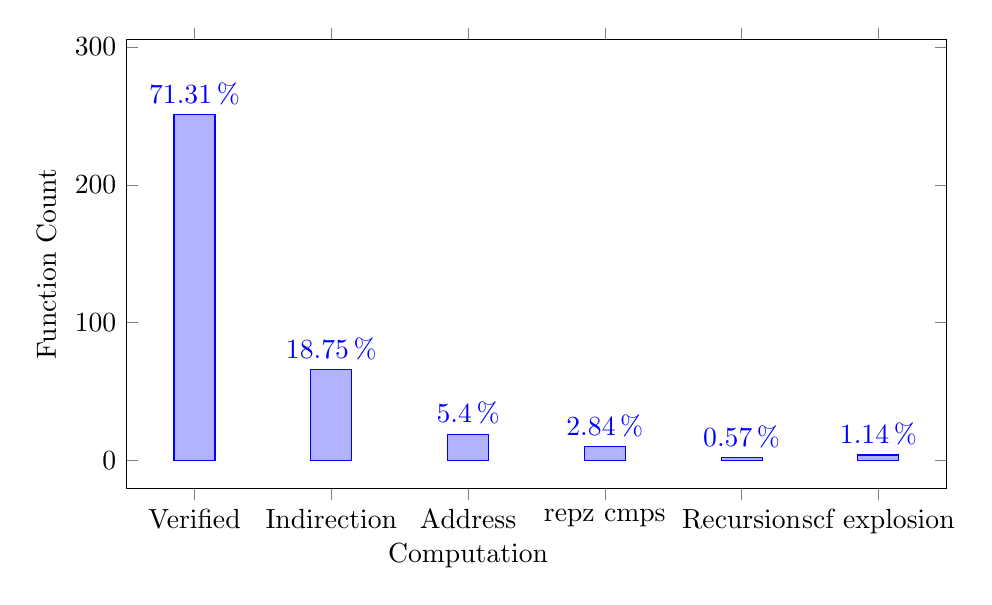
\begin{tikzpicture}
    \begin{axis}[
      width=.99\linewidth,
      height=\axisdefaultheight,
      ybar,
      bar width=0.3,
      point meta=y/3.52,
      % the below sometimes causes build failure when combined with symbolic x coords
      nodes near coords=\pgfmathprintnumber\pgfplotspointmeta\,\%,
      enlarge y limits={value=0.2, upper},
      ymin=-20,
      ylabel=Function Count,
      xticklabels={
        Verified,
        Indirection,
        Address\\Computation,
        \inlineasm{repz cmps},
        Recursion,
        \Glsfmtshort{scf} explosion
      },
      xticklabel style={align=center},
      xtick=data,
    ]
      \addplot coordinates {
        (0, 251)
        (1, 66)
        (2, 19)
        (3, 10)
        (4, 2)
        (5, 4)
      };
    \end{axis}
  \end{tikzpicture}
  \caption{Analyzed Xen functions compared to unverified features}
  \label{fig:unverified}
\end{figure*}

This methodology is currently capable of dealing with \gls{xen-percentage} of the functions present in the aforementioned binaries (see \cref{fig:unverified}).
The supported features include (nested) loops,
subcalls, variable argument lists, jumps into other function bodies,
string instructions with the \inlineasm{rep} prefix, and \gls{simd} instructions.
There is no particular limit on function size.
The average number of instructions per function analyzed is 49.
Some of the functions analyzed have over 300 instructions and over 100 basic blocks.

There are five categories of features not currently supported.
The first and most common, previously mentioned in \cref{sse:cfg_extract},
is \emph{indirection}, accounting for \SI{19}{\percent}.%
\index{indirection}
Indirection involves a call or jump instruction
that loads the target address from a register or memory location
rather than using a static value.
Switch statements and certain uses of \texttt{goto}
are the most common causes of indirect jumps.
Indirect calls generally result from usage of function pointers.
For example, the \lstinline|main| functions of all three verified binaries
used switch statements in loops in the process of parsing command line options.
These statements introduced indirect branches.

The second category involves issues related to generating the \glspl{mrr}.
This step requires solving linear arithmetic over symbolically computed addresses.%
\index{linear arithmetic}
Sometimes, addresses are computed using a combination of arithmetic operators%
\index{operator!arithmetic}
with bitwise logical operators.%
\index{operator!bitwise}
In some of these cases, our translation to \gls{z3} does not produce an answer.
As an example, function \texttt{qcow\_open}
uses the rotate-left function to compute an address.
As another example, function \texttt{AES\_set\_encrypt\_key}
produces addresses that are obtained via combinations of bit-shifting,
bit masking, and \texttt{xor}-ing.
For these cases, separation and enclosure relations cannot be generated.

The instruction \texttt{repz cmps} is currently not supported for technical reasons.
It is the assembly equivalent of the function \texttt{strncmp},
but instead writes its result to a flag.
Various other string-related instructions with the \texttt{rep} prefix are supported,
however.

The two recursive functions encountered in the analyzed Xen binaries
both perform file-system-like tasks.
Functions \lstinline|do_chmod| and \lstinline|do_ls|
are similar to the permission-setting \lstinline|chmod| utility
and the directory-displaying \lstinline|ls|, respectively.

The final category is functions whose \gls{scf} explodes.
The issue can occur when the pattern in \cref{fig:ex_nonopt} shows up extensively or when while loops have multiple entry points.

\Cref{func-counts} provides an overview of the verification effort.
The table shows the absolute counts of functions verified
as well as the total number of instructions for those functions.
Alongside that information is the number of functions with loops
that were verified and how many manual lines of proof were required in total.
The vast majority of those manual proof lines were related to the loop count.
Meanwhile, a comparison with those functions not verified
can be found in \cref{fig:unverified}.

\section{Summary}
This chapter presented an approach to formal verification of \gls{memuse}
for functions in a disassembled program. As in the previous chapter,
the \gls{memuse} reported for those functions is an overapproximation
of the memory that would be used when actually executing the assembly code.
The approach automatically generates \pgls{fmuc} that includes
\begin{enumerate}
  \item a set of memory regions read from and written to,
  \item preconditions necessary for formal verification,
  \item postconditions that express sanity constraints over the function
  (the return address has not been overwritten,
  callee-saved registers are restored, etc.), and
  \item proof ingredients.
\end{enumerate}
The certificate is loaded into a theorem prover, where it can be verified.
The proof ingredients, combined with custom proof methods,
provide a large degree of automation.
They deal with memory aliasing and provide both the control flow of the function
as well as invariants.

The approach was applied to three binaries produced by the Xen hypervisor build process.
They contain nested loops, complex data structures, variadic functions,
and both internal and external function calls.
A certificate could be generated and verified
for \gls{xen-percentage} of the functions from those binaries.
The amount of user interaction was roughly \num{85} lines of proof code
per \num{1000} lines of assembly code.
The greatest issue was indirect branching,
which could be found in \SI{19}\percent\ of the functions examined.
